\newpage
\section{METHODOLOGY}

\subsection{Requirement Specification}
A software requirement specification is a description of a software system to be develped. It lays out functional and non-functional requirements. It describes what the software product is expected to do and what not to do. It enlists enough and necessary requirements that are required for the project development. It mainly aids to describe the scope of the work and provide a software designers a form of reference.
\subsubsection{Functional Requirement}
The functional requirement specification of the project are mainly categorized as user requirements, security requirements, and device requirement each of which are explained in detail below:
\begin{itemize}
\item User Requirement: User should have account on Facebook and usermust have at least one post needed to analyze the personality.
\item Security Requirement: The user can't have access to the Facebook API. User must provide their own login credentials.
\item Device Requirement: System must be initiated on web-browser.

\end{itemize}
\subsubsection{Non-functional Requirement}
The non-functional requirement of the system can be summarized as follows:
\begin{itemize}
\item Performance: The system shall have a quick, accurate and reliable reuslts.
\item Capacity and Scalability: The system shall be able to store personality computed by the system into the database.
\item Availability: The system shall be avilable to user anytime whenever there is an internet connection.
\item Recovery: In case of malfunctioning or unavailability of server, the system should be able to recover and prevent any data loss or redundancy.
\item Flexibility and Portability: System shall be accessible anytime from any locations. 
\end{itemize}
\subsection{Feabisility Assessment}
\subsubsection{Operational Feasiblility}
\subsubsection{Technical Feasiblility}
\subsubsection{Economic Feasibility}
\subsection{Software Development Approach}
The developed system, being huge and dynnamic nature, may not be developed eefficiently and timely procured with the traditional development approaches like waterfall. Thus to meet the requirements of the system and ensuring the timely delivery and adaptibility for changing requirement, Scrum methodology under the Agile Development method is chosen for the developement of system.


\begin{figure}[!ht]
\centering
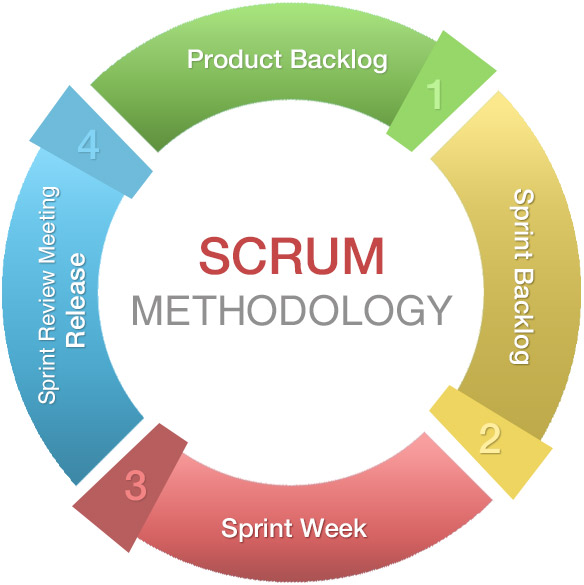
\includegraphics[width = 5 cm]{fig/scrum-chart.jpg}
\caption{scrum software developement cycle}
\label{fig:scrum}
\end{figure}
Scrum is an agile way to manage project. Agile software developlment with Scrum is often perceived as a methodology, but rather than viewing Scrum as methodology, it is often thought as a framework for managing a process. In the agile Scrum world, instead of providing complete, detailed descriptions of how everything is to be done on a project,much of it is left up to Scrum software development team. This is because the team will know best how to solve the problem they are presented. It relies on a self-organizing, cross-functional team. The scrum team is self-organizing in that there is no overall team leader whodecides which person will do which task or how a problem will be solved. This is the issue that are decided by the team as a whole. Besides the team is cross functional, because of which everyone is needed to take a feature from idea to implementation. 

This model suggests that projects progress via a series of sprints. In keeping with an agile methodology, sprints are timeboxed to no more than a month long, most commonly two weeks. It advocates for planning meeting at the start of the sprint, where team members figure out how many items they can commit to and then create a sprint backlog, a list of task to perform during the sprint. During an agile Scrum sprint, the Scrum team takes a small set of features from idea to coded and tested functionality. At the end, these features are coded, tested and integrated into the evolving product or system.

On each day of the sprint, all team members attend a Scrum meeting. During that time, team members share what they worked on the prior day, will work on that day and identify any impediments to progress. The model sees routine scrums as a way to synchronzie the work of team members as they discuss the work of the sprint. At the end of a sprint the sprint review is conducted, during which the team demonstrates the new functionality to any stakeholder who wishes to provide feedback that could influence the next sprint. The feedback loop within Scrum software development may result in changes to the freshly delivered functionality, but it may just as likey result in revising or adding items to the product backlog.

The primary artifact in Scrum development is, the product itself. The Scrum model expects the team to bring the product or system to a potentially shippable state at the end of each Scrum sprint. The product backlog is another artifact of Scrum. This is the complete list of the functionality that remains to be added to the product. The most popular and successful way to create a product backlog using Scrum methodology is to populated it with the user stories, which are short descriptions of functionality described from the prespective of a user or customeer. In Scrum project management, on the first day of a sprint and during the planning meeting, team members create the sprint backlog. The sprint backlog can be thought of as the team's to do list for the sprint whereas the product backlog is a list of features to be built. The sprint backlog is the list of tasks the team needs to perform in order to deliver the functionality it commited to deliver during the sprint. Additional artifacts in the Scrum methodology is the sprint burndown chart which shows the amount of work remaining either in a sprint to determine whether a sprint is on schedule to have all planned work finished by the desired date.

Hence scrum is adpative, has small repeating cycles and there is short-term planning with constant feedback, inspection and adaption and is therefore chosen as the software development methodolgy. Here, project team members can be thought of a software development team and project supervisior as scrum master. The scrum meeting was conducted regulary within the interval of 3 weeks, keeping scrum backlog as well as product backlog and hence the progress in the project was made in the form of sprints whereby the product backlog helped to identify and prioritizes the features to implement in each sprint and the burndown chart helped to keep the project timely on schedule. Whenever the bug was found relating to the feature, it was dealt immediately before marking the feature complete i.2 1-2 sprints ware focused only on Defect backlogs. Each scrum meeting lasted about 15 minutes in which every team member answered three question: What have I done since lastmeeting?, What will I do until next meeting? and What problems do I have? and hence in this way a cycle is continued till product is completely developed.


\subsection{Data Collection}



